\chapter{Спонтанное нарушение суперсимметрии и первый \texorpdfstring{\(SU(5)\)}{SU(5)}-мультиплет}

\lectureoverview{Нарушение симметрии впервые появляется здесь как наглядный факт о спектрах: у атома, инвариантного относительно вращений, уровни углового момента вырождены, тогда как магнитное поле расщепляет их. Затем ферромагнетик преподает более тонкий урок: уравнения могут сохранять симметрию, которой вакуум не обладает. Бесщелевые магноны, условие \(J|0\rangle\neq0\) и ненулевой параметр порядка — это три описания одного и того же явления. Мы переносим эту схему в хиральную суперсимметричную теорию поля, выводим скалярный потенциал \(V=|W'|^2\), устраняя вспомогательное поле \(F\), и различаем суперсимметричные вакуумы и вакуумы с нарушением \(F\). Обсуждение суперсимметрии завершают возникающие при этом энергия вакуума, расщепление бозон--фермион, голдстино, скрытый сектор и супер-Хиггсовский механизм. В заключительной части тема меняется и начинается великое объединение: \(SU(3)\times SU(2)\times U(1)\) блочно вкладывается в \(SU(5)\), чей первый мультиплет материи объединяет лептонный дублет с тремя антидаун-кварками.}

\section{Спектр помнит свою симметрию}

Мы начинаем с атома не только для того, чтобы повторить элементарную квантовую механику. Энергетические уровни и массы частиц — один и тот же тип спектральных данных. Если симметрия заставляет атомные уровни совпадать, то ее нарушение может расщепить их; в теории поля соответствующее утверждение состоит в том, что члены мультиплета частиц могут приобрести разные массы.

Пусть атомное состояние имеет полный угловой момент \(j\), включающий и спиновый, и орбитальный вклады. Относительно любой выбранной оси
\begin{equation}
J_z|j,m\rangle=m\hbar|j,m\rangle,
\qquad
m=-j,-j+1,\ldots,j,
\end{equation}
так что имеется \(2j+1\) состояний. Привычные стрелки из учебников не следует понимать так, будто вектор углового момента буквально имеет в пространстве только \(2j+1\) возможных направлений. Квантуется его компонента вдоль выбранной оси.

В пустом пространстве, инвариантном относительно вращений, нет физической причины предпочесть эту ось. Вращение смешивает состояния внутри мультиплета с общим угловым моментом \(j\), а инвариантность гамильтониана влечет
\begin{equation}
[H,\mathbf J]=0,
\qquad
E_{j,-j}=E_{j,-j+1}=\cdots=E_{j,j}.
\label{eq:l9-degeneracy}
\end{equation}

\begin{classroomqa}
\audiencequestion{Какая симметрия утверждает, что поворот всего атома не может изменить его энергию? \lecturetimestamp{00:05:53}}
\lecturerresponse{Симметрия вращений. Поскольку вращение переводит одну ориентацию углового момента в другую, не изменяя физическую систему, энергия одинакова для всех \(2j+1\) состояний.}
\end{classroomqa}

Теперь приложим магнитное поле \(\mathbf B=B\hat{\mathbf z}\). Взаимодействие
\begin{equation}
H_B=-\boldsymbol{\mu}\cdot\mathbf B
\end{equation}
выделяет компоненту, параллельную полю. Схематически,
\begin{equation}
\Delta E_m\propto mB.
\label{eq:l9-zeeman}
\end{equation}
Уровни с разными \(m\) линейно расходятся при слабом поле, а переходы между ними приводят к расщеплению спектральных линий.

\begin{classroomqa}
\audiencequestion{Как называется расщепление атомных уровней в магнитном поле? \lecturetimestamp{00:07:13}}
\lecturerresponse{Эффект Зеемана. Это прототип всего дальнейшего обсуждения: уровни, сделанные вырожденными симметрией, расходятся, когда фон нарушает эту симметрию.}
\end{classroomqa}

\begin{center}
\begin{tikzpicture}[x=1.05cm,y=0.75cm,>=Latex]
  \draw[thick] (-3,0) -- (-1,0);
  \node[left] at (-3,0) {\(B=0\)};
  \foreach \y/\m in {-1.2/-1,-0.4/0,0.4/1,1.2/2} {
    \draw[thick,teal!70!black] (1,\y) -- (3,\y);
    \node[right] at (3,\y) {\(m=\m\)};
  }
  \draw[->,thick] (-0.5,0) -- (0.6,0);
  \node[above] at (0.05,0) {\(\mathbf B\neq0\)};
\end{tikzpicture}
\end{center}

\section{Ферромагнетик: симметричные законы, асимметричный вакуум}

В простой микроскопической картине ферромагнетика каждому узлу приписывается небольшой магнитный момент. Если соседние моменты понижают свою энергию, становясь параллельными, то низкотемпературная фаза является ферромагнитной. Если предпочтительна антипараллельная ориентация, результатом будет антиферромагнетик. Сильные тепловые или квантовые флуктуации могут, напротив, размыть любую суммарную намагниченность.

Предположим, что ферромагнетик заполняет весь мир и устанавливается в состояние с однородно выровненными моментами. Его внутреннее магнитное поле расщепляет уровни атома точно так же, как это делало бы внешне наложенное поле. Однако есть решающее различие. Фундаментальные взаимодействия не выделяют ни север, ни восток, ни какое-либо другое направление. Любая однородно повернутая конфигурация имеет одну и ту же энергию:
\begin{equation}
\mathbf M(\mathbf x)=M_0\hat{\mathbf n},
\qquad
\hat{\mathbf n}\in S^2.
\label{eq:l9-ferromagnetic-vacua}
\end{equation}
Уравнения инвариантны относительно вращений, но одно конкретное основное состояние выбирает одно \(\hat{\mathbf n}\). Это спонтанное, а не явное нарушение симметрии.

Житель, составленный из возбуждений этой среды, не может схватить всю Вселенную и повернуть ее. Поэтому локально выбранное направление выглядит столь же фундаментальным, как внешнее поле. Атом по-прежнему видит ту же структуру уровней, причем его угловой момент разрешается вдоль \(\hat{\mathbf n}\), а не вдоль внешне названной оси \(z\). Вопрос в том, как внутренний наблюдатель мог бы обнаружить, что кажущаяся асимметрия принадлежит состоянию, а не законам.

\subsection{Критерий Голдстоуна}

Однородный поворот каждого момента переводит систему из одного вакуума в формуле ~\eqref{eq:l9-ferromagnetic-vacua} в другой и не требует энергии. Пусть вместо этого ориентация меняется в пространстве очень медленно. Тогда соседние моменты воздействуют друг на друга, и искажение распространяется как спиновая волна, кванты которой — магноны. Когда длина волны стремится к бесконечности, конфигурация приближается к однородному повороту, так что ее энергия возбуждения стремится к нулю:
\begin{equation}
k=\frac{2\pi}{\lambda}\longrightarrow0
\quad\Longrightarrow\quad
E(k)\longrightarrow0.
\label{eq:l9-gapless-magnon}
\end{equation}
Два жителя могут слегка возмутить соседние моменты, послать такие волны через среду и измерить эту сколь угодно малую энергию. Этот эксперимент обнаруживает спонтанное нарушение, хотя они не могут повернуть весь мир.

\editorialnote{Ферромагнитный магнон бесщелевой, но обычно имеет нерелятивистский квадратичный закон дисперсии \(E\propto k^2\), а не релятивистское соотношение \(E\propto|k|\). В лекции слово безмассовый используется в физически существенном смысле исчезающей щели. И то и другое — голдстоуновские моды.}

Та же идея применима к непрерывным внутренним симметриям, включая калибровочные и ароматовые группы физики частиц. Однако когда нарушенная симметрия является калибровочной, голдстоуновская мода не остается независимой безмассовой частицей.

\begin{classroomqa}
\audiencequestion{Что происходит, когда спонтанное нарушение симметрии сочетается с калибровочной инвариантностью? \lecturetimestamp{00:15:56}}
\lecturerresponse{Голдстоуновский бозон дает калибровочному полю дополнительную поляризацию. Калибровочный бозон становится массивным; это механизм Хиггса, к которому мы вернемся в гравитационной аналогии.}
\end{classroomqa}

\section{Три эквивалентных признака нарушения}

Теперь ферромагнетик можно описать тремя взаимно дополняющими языками.

\paragraph{Вырожденные вакуумы.}
Каждой ориентации \(\hat{\mathbf n}\) соответствует одно состояние минимальной энергии. Физика реализуется в одном выбранном члене этого семейства, хотя симметрия связывает их все.

\paragraph{Генератор, который не уничтожает вакуум.}
Пусть \(J_a\) — генератор вращений. Конечное преобразование имеет вид
\begin{equation}
U(\epsilon)=e^{-i\epsilon J_a},
\end{equation}
и \(J_a|0\rangle\) пропорционально бесконечно малому изменению вакуума, а не всему повернутому состоянию.

\begin{classroomqa}
\audiencequestion{Каковы генераторы симметрии вращений? \lecturetimestamp{00:17:29}}
\lecturerresponse{Компоненты полного углового момента. Мы обозначаем их \(J_a\), потому что они поворачивают все состояние, а не только один атом.}
\end{classroomqa}

Для ненарушенного генератора выполняется
\begin{equation}
J_a|0\rangle=0.
\label{eq:l9-unbroken-generator}
\end{equation}
Для нарушенного генератора, напротив, имеем
\begin{equation}
J_a|0\rangle\neq0.
\label{eq:l9-broken-generator}
\end{equation}

\begin{classroomqa}
\audiencequestion{Если \(J_a|0\rangle\) ненулево, означает ли это просто тот же самый вакуум? \lecturetimestamp{00:19:43}}
\lecturerresponse{Нет. Оно задает бесконечно малую разность между выбранным вакуумом и слегка повернутым. Физически эта разность представляет собой голдстоуновское возбуждение с бесконечно большой длиной волны.}
\end{classroomqa}

\begin{classroomqa}
\audiencequestion{Изменяет ли этот бесконечно малый поворот энергию? \lecturetimestamp{00:20:14}}
\lecturerresponse{Нет. Повернутый вакуум вырожден с исходным, поэтому голдстоуновское состояние с нулевым импульсом имеет нулевую энергию.}
\end{classroomqa}

Схематически,
\begin{equation}
J_a|0\rangle
\sim
|\pi_a,\mathbf k=0\rangle,
\label{eq:l9-generator-goldstone}
\end{equation}
где \(\pi_a\) обозначает голдстоуновскую моду, связанную с нарушенным генератором.

\paragraph{Ненулевой параметр порядка.}
Локальная намагниченность \(\mathbf M(\mathbf x)\) — это поле. В термически или квантово-разупорядоченной фазе,
\begin{equation}
\langle\mathbf M\rangle=0,
\end{equation}
и вакуум не выбирает направления. В упорядоченной фазе,
\begin{equation}
\langle M_i\rangle\neq0
\quad\text{for at least one component }i,
\label{eq:l9-magnetization-order}
\end{equation}
так что вращение смешивает эту ненулевую компоненту с остальными. Вырожденные вакуумы, нарушенный генератор и ненулевой параметр порядка — это три схемы, которые мы перенесем в суперсимметрию.

\section{Напоминание о хиральном мультиплете}

Самый простой четырехмерный пример содержит один комплексный скаляр, один фермион Вейля и один вспомогательный комплексный скаляр. В хиральных координатах,
\begin{equation}
y^\mu=x^\mu+i\bar\theta\bar\sigma^\mu\theta,
\end{equation}
хиральное суперполе можно схематически разложить как
\begin{equation}
\Phi(y,\theta)=
\phi(y)+\sqrt2\,\theta\psi(y)+\theta^2F(y).
\label{eq:l9-chiral-expansion}
\end{equation}
В лекции стандартный множитель \(\sqrt2\) опущен; начиная с этого места мы его включаем, чтобы коэффициенты компонент были стандартными. Хиральное суперполе по самой своей природе комплексно: наложение условия вещественности не сохраняется при его преобразовании суперсимметрии.

Суперсимметричное кинетическое действие имеет вид
\begin{equation}
S_{\mathrm{kin}}
=
\int d^4x\,d^4\theta\,
\Phi^\dagger\Phi.
\label{eq:l9-kahler-action}
\end{equation}
Интегрирование по грассмановым переменным выделяет коэффициент при \(\theta^2\bar\theta^2\). При сигнатуре метрики с преобладанием минусов компонентный результат таков:
\begin{equation}
\mathcal L_{\mathrm{kin}}
=
\partial_\mu\phi^\ast\,\partial^\mu\phi
+i\bar\psi\bar\sigma^\mu\partial_\mu\psi
+F^\ast F.
\label{eq:l9-chiral-kinetic}
\end{equation}
Первые два члена описывают распространение скаляра и фермиона. Последний не содержит производных и потому не описывает распространение никакой частицы.

\begin{figure}[H]
\centering
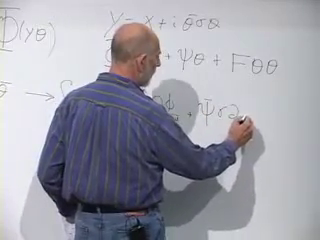
\includegraphics[width=0.76\textwidth]{lecture_09_figure_02.png}
\lectureframe{00:27:36.000}
\caption{Хиральная координата и приведенное выше компонентное разложение: скалярный, фермионный и вспомогательный члены.}
\end{figure}

\section{Что выделяет интеграл \texorpdfstring{\(d^2\theta\)}{d2-theta}}

Взаимодействия и массы возникают из голоморфной функции \(W(\Phi)\), суперпотенциала:
\begin{equation}
S_W
=
\int d^4x
\left[
\int d^2\theta\,W(\Phi)
+\mathrm{h.c.}
\right].
\label{eq:l9-superpotential-action}
\end{equation}
Хиральное выражение не имеет независимой зависимости от \(\bar\theta\), поэтому интегрирование по всем четырём нечётным координатам дало бы нуль. Интеграл \(d^2\theta\) вместо этого выделяет его компоненту \(\theta^2\).

Чтобы увидеть комбинаторику до перехода к общей функции, положим \(W(\Phi)=\Phi^n\). В
\begin{equation}
(\phi+\sqrt2\,\theta\psi+\theta^2F)^n,
\end{equation}
есть два способа получить ровно две \(\theta\). Можно выбрать один \(F\theta^2\) или выбрать два фермионных множителя.

\begin{classroomqa}\audiencequestion{Сколько членов содержат один выбранный \(F\theta^2\) и в остальном только скаляры: \(n-1\) или \(n\)? \lecturetimestamp{00:31:33}}
\lecturerresponse{Их \(n\). Любой из \(n\) множителей может дать \(F\theta^2\); оставшиеся \(n-1\) множителей дают \(\phi\). Вклад равен \(nF\phi^{n-1}\).}
\end{classroomqa}

\begin{classroomqa}\audiencequestion{Сколькими способами два множителя могут дать два фермиона? \lecturetimestamp{00:32:26}}
\lecturerresponse{Есть \(\binom n2=n(n-1)/2\) неупорядоченных выборов. Грассманово свёртывание фиксирует соответствующий член \(\psi\psi\).}
\end{classroomqa}

Итак, в используемом на лекции обозначении с подавленными коэффициентами,
\begin{equation}
\int d^2\theta\,\Phi^n+\mathrm{h.c.}
\;\leadsto\;
nF\phi^{n-1}
-\frac{n(n-1)}{2}\phi^{n-2}\psi\psi
+\mathrm{h.c.}
\label{eq:l9-power-extraction}
\end{equation}
Показанный здесь знак минус следует из стандартного нормированного разложения и грассмановых соглашений; при изменении соглашений формальные знаки могут сдвинуться.

\begin{classroomqa}\audiencequestion{Что произошло с членом \(\phi^n\), который вообще не содержит \(\theta\)? \lecturetimestamp{00:33:10}}
\lecturerresponse{Он присутствует в произведении, но \(d^2\theta\) его отбрасывает. Стрелка означает, что интегрирование выделяет коэффициент при \(\theta^2\); это не равенство полных выражений.}
\end{classroomqa}

\begin{figure}[H]
\centering
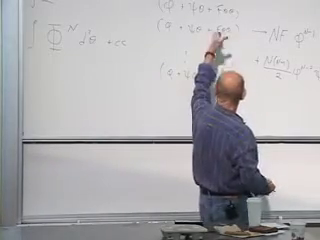
\includegraphics[width=0.82\textwidth]{lecture_09_figure_03.png}
\lectureframe{00:33:38.000}
\caption{Повторяющиеся множители суперполя и стрелка, которая выделяет, а не приравнивает, их компоненту с двумя \(\theta\).}
\end{figure}

Суммирование степеней с произвольными коэффициентами превращает комбинаторные множители в производные:
\begin{equation}
\int d^2\theta\,W(\Phi)+\mathrm{h.c.}
\;\leadsto\;
F W'(\phi)
-\frac12 W''(\phi)\psi\psi
+\mathrm{h.c.}
\label{eq:l9-W-components}
\end{equation}

\begin{classroomqa}\audiencequestion{Почему фермионный член содержит \(\phi^{n-2}\), а не \(\phi^{n-1}\)? \lecturetimestamp{00:36:32}}
\lecturerresponse{Два множителя уже дали фермионы, оставив \(n-2\) скалярных множителей. Коэффициент равен половине второй производной \(W''(\phi)\).}
\end{classroomqa}

Фермионный член важен: он даёт массу, когда \(W''\) является константой, и взаимодействие Юкавы, когда \(W''\) зависит от \(\phi\). Однако для анализа вакуума непосредственную информацию несёт вспомогательный член \(FW'\).

\section{Исключение вспомогательного поля}

Соберём члены, содержащие \(F\):
\begin{equation}
\mathcal L_F
=
F^\ast F
+F W'(\phi)
+F^\ast \overline{W'(\phi)}.
\label{eq:l9-LF}
\end{equation}
Поскольку \(\partial_\mu F\) отсутствует, полное уравнение Эйлера--Лагранжа
\begin{equation}
\partial_\mu
\frac{\partial\mathcal L}{\partial(\partial_\mu F)}
-
\frac{\partial\mathcal L}{\partial F}
=0
\end{equation}
сразу сводится к алгебраическому уравнению. Если рассматривать \(F\) и \(F^\ast\) как независимые переменные, получаем
\begin{align}
\frac{\partial\mathcal L_F}{\partial F}
&=F^\ast+W'(\phi)=0,
&
\frac{\partial\mathcal L_F}{\partial F^\ast}
&=F+\overline{W'(\phi)}=0,
\label{eq:l9-F-eom}
\end{align}
и, следовательно,
\begin{equation}
F^\ast=-W'(\phi),
\qquad
F=-\overline{W'(\phi)}.
\label{eq:l9-F-solution}
\end{equation}

\begin{figure}[H]
\centering
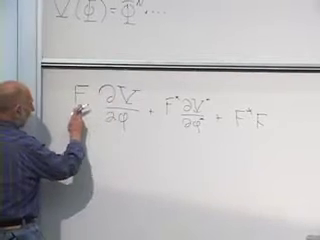
\includegraphics[width=0.82\textwidth]{lecture_09_figure_04.png}
\lectureframe{00:39:40.000}
\caption{Полное выражение для вспомогательного поля и его алгебраическое уравнение движения, видимые вместе после того, как доска оказывается незаслонённой.}
\end{figure}

\begin{classroomqa}\audiencequestion{Эту производную следует брать по \(\phi\), а не по сопряжённому полю, написанному на доске? \lecturetimestamp{00:41:21}}
\lecturerresponse{Да. Это исправление восстанавливает сопряжённую пару в уравнении~\eqref{eq:l9-F-eom}: \(F^\ast=-W'(\phi)\) и \(F=-\overline{W'(\phi)}\).}
\end{classroomqa}

Подстановка в уравнение~\eqref{eq:l9-LF} даёт
\begin{equation}
\mathcal L_F\big|_{\mathrm{on\ shell}}
=-|W'(\phi)|^2.
\end{equation}
Поскольку скалярный лагранжиан имеет вид кинетическая энергия минус потенциальная энергия, обычный скалярный потенциал равен
\begin{equation}
\boxed{V(\phi,\phi^\ast)=|W'(\phi)|^2\ge0.}
\label{eq:l9-F-potential}
\end{equation}
Этот \(V\) не является суперпотенциалом. Обозначение \(W\) мы сохраняем для голоморфной функции в суперпространстве, а \(V\) — для обычной потенциальной энергии.

\subsection{Два непосредственных примера}

При точных общепринятых нормировках,
\begin{equation}
\begin{gathered}
W(\Phi)=\frac12m\Phi^2,\\
W'(\phi)=m\phi,
\qquad V=|m|^2|\phi|^2.
\end{gathered}
\label{eq:l9-quadratic-W}
\end{equation}
Тот же член даёт массу фермиона
\(-\tfrac12m\psi\psi+\mathrm{h.c.}\), так что массы скаляра и фермиона совпадают до нарушения суперсимметрии.

Для
\begin{equation}
W(\Phi)=\frac{g}{3}\Phi^3,
\end{equation}
получаем
\begin{equation}
\begin{gathered}
W'(\phi)=g\phi^2,
\qquad V=|g|^2|\phi|^4,\\
\mathcal L_{\mathrm{Yukawa}}
=-g\phi\psi\psi+\mathrm{h.c.}
\end{gathered}
\label{eq:l9-cubic-W}
\end{equation}
Четырёхскалярная вершина описывает рассеяние двух скаляров, тогда как член Юкавы является её суперсимметричным партнёром.

\section{Два вида вакуума}

Вакуум — это постоянная конфигурация поля в минимуме \(V\); члены с производными обращаются в нуль. Поскольку выражение в уравнении~\eqref{eq:l9-F-potential} неотрицательно, возможны два случая.

\subsection{Минимум с нулевой энергией}

Если некоторое \(\phi_0\) удовлетворяет
\begin{equation}
W'(\phi_0)=0,
\end{equation}
то
\begin{equation}
V(\phi_0)=0,
\qquad
\langle F\rangle=0.
\label{eq:l9-unbroken-F}
\end{equation}
Вакуум суперсимметричен. Это аналог исчезающей намагниченности: никакая вспомогательная компонента не выделила направление в суперпространстве.

\subsection{Поднятый минимум}

Если уравнения
\begin{equation}
W'(\phi)=0
\label{eq:l9-F-flatness}
\end{equation}
не имеют в минимуме одновременного решения, то
\begin{equation}
V_{\min}>0,
\qquad
\langle F\rangle\neq0,
\label{eq:l9-broken-F}
\end{equation}
и суперсимметрия спонтанно нарушена. Действие остаётся суперсимметричным; его состояние с наименьшей энергией — нет.

\begin{figure}[H]
\centering
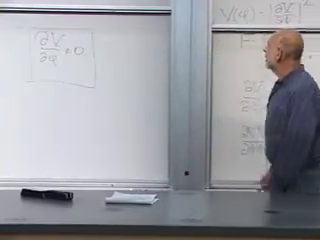
\includegraphics[width=0.88\textwidth]{lecture_09_figure_05.png}
\lectureframe{00:52:09.960}
\caption{На доске одновременно остаются положительный потенциал, уравнение для \(F\) и условие на вакуум, при этом симметричные уравнения отличены от несимметричного решения.}
\end{figure}

Утверждение о параметре порядка можно сделать точным с помощью преобразования фермиона:
\begin{equation}
\delta\psi_\alpha
=
i\sqrt2
(\sigma^\mu\bar\epsilon)_\alpha\partial_\mu\phi
+\sqrt2\,\epsilon_\alpha F.
\label{eq:l9-fermion-transformation}
\end{equation}
Для однородного вакуума член с производной исчезает. Если
\(\langle F\rangle\neq0\), суперсимметрия сдвигает фермион на ненулевую константу, так что вакуум не может быть инвариантным.\editorialnote{Уравнение~\eqref{eq:l9-fermion-transformation} — это стандартная компонентная форма, в которой явно выражено утверждение лекции о том, что компоненты суперполя преобразуются друг в друга.}

Тот же вывод следует из супералгебры. В системе покоя,
\begin{equation}
\{Q_\alpha,Q_{\dot\alpha}^\dagger\}
=2\sigma^0_{\alpha\dot\alpha}H.
\end{equation}
Взятие вакуумного среднего выражает энергию вакуума как сумму норм суперзарядов, действующих на вакуум:
\begin{equation}
E_0\ge0,
\qquad
E_0=0
\ \Longleftrightarrow\
Q_\alpha|0\rangle
=Q_{\dot\alpha}^\dagger|0\rangle=0.
\label{eq:l9-algebra-vacuum-energy}
\end{equation}
Следовательно, положительная энергия вакуума и спонтанное нарушение суперсимметрии — две стороны одного и того же утверждения о жёсткой суперсимметрии.

\begin{center}
\begin{tikzpicture}[x=1.2cm,y=1.0cm,>=Latex]
  \draw[->] (-3,0) -- (-0.2,0) node[right] {\(\phi\)};
  \draw[->] (-2.8,-0.15) -- (-2.8,2.1) node[above] {\(V\)};
  \draw[thick,teal!75!black,domain=-2.5:-0.5,samples=60]
    plot (\x,{0.65*(\x+1.5)^2});
  \fill (-1.5,0) circle (2pt);
  \node[below] at (-1.5,0) {\(F=0\)};
  \draw[->] (0.4,0) -- (3.2,0) node[right] {\(\phi\)};
  \draw[->] (0.6,-0.15) -- (0.6,2.1) node[above] {\(V\)};
  \draw[thick,orange!85!black,domain=0.9:2.9,samples=60]
    plot (\x,{0.55*(\x-1.9)^2+0.65});
  \fill (1.9,0.65) circle (2pt);
  \draw[dashed] (0.6,0.65) -- (1.9,0.65);
  \node[below] at (1.9,0.65) {\(F\neq0\)};
\end{tikzpicture}
\end{center}

\editorialnote{Минимальный пример — \(W=f\Phi\), для которого \(W'=f\) никогда не обращается в нуль и \(V=|f|^2\). Этот однополевой пример имеет плоское скалярное направление; реалистичное устойчивое нарушение по \(F\)-члену обычно реализуют с несколькими хиральными полями, как в скрытых секторах типа O'Raifeartaigh.}

\section{Что порождает нарушенная суперсимметрия}

\subsection{Расщепление масс}

Ферромагнитная аналогия теперь снова становится спектральной. Слабое внутреннее магнитное поле расщепляет атомные уровни, не лишая атом его идентичности. Аналогично, слабо передаваемый параметр порядка нарушения суперсимметрии расщепляет бозоны и фермионы, которые иначе принадлежали бы одному супермультиплету.

\begin{classroomqa}\audiencequestion{Какие частицы суперсимметрия преобразует друг в друга и потому теряют вырождение по массе, когда вакуум её нарушает? \lecturetimestamp{00:51:40}}
\lecturerresponse{Бозоны и фермионы. Их массы не обязаны оставаться равными, когда состояние больше не инвариантно относительно преобразования, которое их связывает.}
\end{classroomqa}

Расщепление не создаётся одним только \(\langle F\rangle\); оно зависит от взаимодействий, которые передают нарушение видимым полям. Если эти взаимодействия слабы, видимые частицы остаются узнаваемыми, а расщепления малы по сравнению с масштабами великого объединения или Планка. Если бы они были сильными, аналогом был бы атом, настолько искажённый огромным магнитным полем, что он превратился бы в длинный неузнаваемый объект.

\subsection{Голдстино}

Для обычного нарушенного генератора \(J|0\rangle\) даёт бозонное состояние Голдстоуна. Суперзаряд фермионен и переводит бозонные состояния в фермионные. Поскольку вакуум считается бозонным, нарушенный суперзаряд создаёт фермионное состояние с нулевой энергией:
\begin{equation}
Q_\alpha|0\rangle
\sim
|\widetilde G_\alpha,\mathbf k=0\rangle.
\label{eq:l9-goldstino}
\end{equation}
Его распространяющееся продолжение — безмассовый вейлевский фермион, голдстоуновский фермион, или голдстино.

\begin{classroomqa}
\audiencequestion{Если преобразование суперсимметрии не оставляет вакуум неизменным, какое новое состояние оно порождает? \lecturetimestamp{00:53:24}}
\lecturerresponse{Безмассовый фермион. Обычная картина теоремы Голдстоуна сохраняется, но фермионный генератор переводит бозонный вакуум в голдстино.}
\end{classroomqa}

Поэтому спонтанное нарушение жёсткой суперсимметрии имеет два неизбежных признака:
\begin{equation}
\boxed{
V_{\min}>0
\qquad\text{and}\qquad
\text{a massless goldstino}.
}
\label{eq:l9-rigid-breaking-signatures}
\end{equation}

\section{Скрытый сектор}

Удобно называть атом и ферромагнетик двумя секторами. В ферромагнетике возникает параметр порядка; атом ощущает только поле, передаваемое от него. Когда связь слаба, манипулирование атомом едва возбуждает магнон и даёт очень мало прямого доступа к магнитной среде. Тогда ферромагнетик скрыт, хотя о его присутствии судят по небольшим расщеплениям спектра.

При построении суперсимметричных моделей используется тот же язык. Дополнительные поля в скрытом секторе приобретают ненулевые средние значения \(F\)- или \(D\)-членов. Взаимодействия, называемые механизмом передачи, передают это нарушение в видимый сектор и порождают мягкие массы суперпартнёров. Слабая передача объясняет, как видимая теория может оставаться приблизительно суперсимметричной при гораздо более высоком фундаментальном масштабе, не демонстрируя при этом точного низкоэнергетического бозон--фермионного вырождения.

Построение не является автоматическим. Требуются дополнительные поля, устойчивый вакуум, в котором суперсимметрия нарушена, и контролируемый механизм передачи. Поэтому в лекции реалистическое нарушение суперсимметрии описывается как сложное и несколько искусственное, а не как единственное неизбежное следствие минимальной модели.

\section{Гравитация меняет оба признака}

\subsection{Энергия вакуума становится источником}

Без гравитации сдвиг всех энергий на константу не меняет результатов негравитационных экспериментов. При наличии гравитации плотность энергии вакуума входит в уравнение Эйнштейна как космологическая постоянная. Положительное \(V_{\min}\) вызывает ускоренное расширение. Если бы этот масштаб был сравним с масштабом физики частиц, необходимым для масс суперпартнёров, возникающая кривизна была бы неизмеримо больше наблюдаемой.

\begin{classroomqa}
\audiencequestion{Что делает с миром положительная ненулевая энергия вакуума, когда учитывается гравитация? \lecturetimestamp{01:00:40}}
\lecturerresponse{Она действует как космологическая постоянная и вызывает ускоренное расширение. При обычных масштабах физики частиц этот эффект был бы недопустимо велик.}
\end{classroomqa}

Локальная суперсимметрия, или супергравитация, изменяет формулу положительной суммы квадратов. Для ориентира стандартный потенциал \(N=1\) \(F\)-члена имеет вид
\begin{equation}
\begin{aligned}
V_F={}&e^{K/M_P^2}
\left(
K^{i\bar j}D_iW\,D_{\bar j}\overline W
-\frac{3|W|^2}{M_P^2}
\right),\\
D_iW={}&\partial_iW+\frac{\partial_iK}{M_P^2}W.
\end{aligned}
\label{eq:l9-sugra-potential}
\end{equation}
Из-за отрицательного члена положительная энергия, возникающая при нарушении суперсимметрии, в принципе может быть частично скомпенсирована. Оставшаяся часть может быть малой космологической постоянной.

\editorialnote{В лекции намеренно даётся лишь схематическая поправка, и прямо ставится под вопрос, где в формуле должна стоять масса Планка. Формула~\eqref{eq:l9-sugra-potential} даёт общепринятое выражение для хиральных мультиплетов с потенциалом Кэлера \(K\); калибровочные \(D\)-члены добавили бы ещё один неотрицательный вклад. Она не объясняет наблюдаемое крошечное значение, что и остаётся проблемой космологической постоянной.}

\subsection{Механизм супер-Хиггса}

Второй гравитационный эффект проще всего понять, подсчитав поляризации. Массивная частица со спином \(j\) имеет в системе покоя \(2j+1\) спиновых состояний.

\begin{classroomqa}
\audiencequestion{Сколько спиновых состояний имеет массивная частица со спином \(j\)? \lecturetimestamp{01:05:16}}
\lecturerresponse{\(2j+1\) спиновых состояний. В частности, массивная частица со спином один имеет три состояния, тогда как безмассовый калибровочный бозон имеет только спиральности \(+1\) и \(-1\).}
\end{classroomqa}

Различие носит кинематический характер. Массивную частицу можно лоренцевым бустом перевести в систему покоя, а затем заставить двигаться в другом направлении, сохранив ориентацию её спина, так что должны существовать все проекции. Безмассовую частицу нельзя ни обогнать, ни привести в состояние покоя. Поэтому у неё возможны только две крайние спиральности.

Для электрослабого калибровочного поля имеем
\begin{equation}
\underbrace{(+1,-1)}_{\text{massless vector}}
+
\underbrace{(0)}_{\text{Goldstone}}
\longrightarrow
\underbrace{(+1,0,-1)}_{\text{massive vector}}.
\label{eq:l9-higgs-count}
\end{equation}

\begin{classroomqa}
\audiencequestion{Откуда берётся продольная поляризация у массивного \(W\) или \(Z\)? \lecturetimestamp{01:08:50}}
\lecturerresponse{От бозона Голдстоуна. Он поглощается калибровочным полем и дополняет представление массивной частицы со спином один до трёх состояний.}
\end{classroomqa}

В гравитации есть безмассовый гравитон со спином два. Его суперсимметрический партнёр — безмассовый гравитино со спином \(\tfrac32\).

\begin{classroomqa}
\audiencequestion{Каков спин гравитона и, следовательно, его суперпартнёра? \lecturetimestamp{01:10:24}}
\lecturerresponse{У гравитона спин \(2\); спин фермионного партнёра отличается на половину и равен \(3/2\).}
\end{classroomqa}

Безмассовое гравитино имеет спиральности \(\pm\tfrac32\), тогда как массивное гравитино должно также иметь \(\pm\tfrac12\). Голдстино как раз и предоставляет эти недостающие состояния:
\begin{equation}
\begin{gathered}
\underbrace{\left(+\frac32,-\frac32\right)}_{\text{massless gravitino}}
\oplus
\underbrace{\left(+\frac12,-\frac12\right)}_{\text{goldstino}}\\
\Downarrow\\
\underbrace{\left(+\frac32,+\frac12,-\frac12,-\frac32\right)}_{\text{massive gravitino}}.
\end{gathered}
\label{eq:l9-super-higgs}
\end{equation}
Это супер-хиггсовский механизм. Как только суперсимметрия становится локальной, голдстино поглощается и больше не появляется как независимая безмассовая частица. Образовавшееся гравитино взаимодействует гравитационно, и поэтому его трудно рождать.

\section{Смена темы: почему \texorpdfstring{\(SU(5)\)}{SU(5)}?}

Теперь формализм суперсимметрии уступает место великому объединению. Калибровочная группа Стандартной модели имеет вид
\begin{equation}
G_{\mathrm{SM}}
=SU(3)_c\times SU(2)_L\times U(1)_Y.
\label{eq:l9-sm-group}
\end{equation}
Её три множителя по отдельности отвечают за цвет, слабый изоспин и слабый гиперзаряд. Вопрос объединения состоит в том, является ли это произведение сохранившейся подгруппой одной более крупной простой группы, так что кажущиеся отдельными мультиплеты частиц и калибровочные взаимодействия оказываются частями единой структуры. Минимальный кандидат, рассматриваемый здесь, — \(SU(5)\).

\subsection{Элементы группы и генераторы}

Для \(U\in SU(N)\) имеем
\begin{equation}
U^\dagger U=\mathbf1,
\qquad
\det U=1.
\label{eq:l9-SUN-def}
\end{equation}
Первое условие выражает унитарность; второе соответствует слову «special». Запишем бесконечно малый элемент в виде
\begin{equation}
U=\mathbf1+i\epsilon G+\mathcal O(\epsilon^2).
\label{eq:l9-infinitesimal-U}
\end{equation}
Унитарность требует
\begin{equation}
G^\dagger=G,
\end{equation}
а условие
\begin{equation}
\det e^{i\epsilon G}
=e^{i\epsilon\operatorname{tr}G}=1
\end{equation}
требует
\begin{equation}
\operatorname{tr}G=0.
\end{equation}
Следовательно, генераторы — это эрмитовы матрицы с нулевым следом.

Эрмитова матрица размера \(N\times N\) содержит \(N^2\) вещественных параметров: \(N\) вещественных диагональных элементов и \(N(N-1)/2\) комплексных внедиагональных элементов. Условие нулевого следа убирает один из них. Поэтому
\begin{equation}
\dim SU(N)=N^2-1,
\qquad
\dim SU(5)=24.
\label{eq:l9-SU5-dimension}
\end{equation}
Для сравнения, у \(SU(2)\) три генератора Паули, а у \(SU(3)\) — восемь цветовых генераторов.

\section{Блоки Стандартной модели внутри \texorpdfstring{\(SU(5)\)}{SU(5)}}

Разобьём пятимерное пространство на слабый двумерный блок и цветовой трёхмерный блок:
\begin{equation}
\mathbf5=\mathbf2\oplus\mathbf3.
\end{equation}
Вложенные генераторы имеют вид
\begin{align}
T^a_L
&=
\begin{pmatrix}
\tfrac12\tau^a&0\\
0&0_{3\times3}
\end{pmatrix},
&& a=1,2,3,
\label{eq:l9-SU2-block}\\
T^A_c
&=
\begin{pmatrix}
0_{2\times2}&0\\
0&\tfrac12\lambda^A
\end{pmatrix},
&& A=1,\ldots,8.
\label{eq:l9-SU3-block}
\end{align}
Матрицы Паули \(\tau^a\) порождают слабую \(SU(2)\); матрицы Гелл-Манна \(\lambda^A\) порождают цветовую \(SU(3)\). Поскольку блоки не перекрываются, эти две подгруппы коммутируют.

Ещё один диагональный генератор пропорционален единичной матрице внутри каждого блока и поэтому коммутирует с обеими. В фундаментальном представлении одна удобная конвенция для удвоенного гиперзаряда имеет вид
\begin{equation}
T_Y^{(\mathbf5)}=
\operatorname{diag}
\left(
1,1,-\frac23,-\frac23,-\frac23
\right).
\label{eq:l9-hypercharge-generator}
\end{equation}
Его след равен нулю:
\begin{equation}
1+1-3\left(\frac23\right)=0.
\end{equation}
Сопряжённое представление материи имеет противоположные собственные значения,
\begin{equation}
Y_{\overline{\mathbf5}}
=
\operatorname{diag}
\left(
-1,-1,\frac23,\frac23,\frac23
\right),
\label{eq:l9-fivebar-hypercharge}
\end{equation}
именно они и выписаны в лекции в столбце matter. Общий знак и нормировка условны; здесь используется конвенция Стандартной модели
\begin{equation}
Q=T_3+\frac{Y}{2}.
\label{eq:l9-charge}
\end{equation}
Уравнения~\eqref{eq:l9-SU2-block}--\eqref{eq:l9-hypercharge-generator} показывают
\begin{equation}
SU(3)_c\times SU(2)_L\times U(1)_Y
\subset SU(5).
\end{equation}

Три слабых генератора, восемь цветовых генераторов и один генератор гиперзаряда составляют \(12\) из \(24\) генераторов \(SU(5)\).\editorialnote{Остальные двенадцать располагаются во внедиагональных блоках \(2\times3\) и \(3\times2\). Их калибровочные бозоны переводят кваркоподобные и лептоноподобные компоненты друг в друга; в этом состоит структурный источник взаимодействий, изменяющих барионность и лептонность, которые будут рассмотрены далее.}

\begin{classroomqa}
\audiencequestion{Какие калибровочные частицы соответствуют генераторам знакомых подгрупп? \lecturetimestamp{01:31:05}}
\lecturerresponse{Восемь генераторов \(SU(3)\) дают восемь глюонов. Три генератора \(SU(2)\) дают слабые калибровочные поля, которые после электрослабого смешивания становятся \(W^\pm\) и частью \(Z\)-фотонной системы; поле \(U(1)\) даёт другую нейтральную комбинацию.}
\end{classroomqa}

\section{Одно семейство на языке левохиральных полей}

Сосредоточимся на первом поколении; та же схема повторяется для поколений мюон/чарм/стрэйндж и тау/топ/боттом. Наиболее экономно считать каждое независимое вейлевское поле левохиральным. Правохиральные частицы представляются их левохиральными зарядово-сопряжёнными полями:
\begin{equation}
Q_L=(u_L,d_L),\quad
L_L=(\nu_{eL},e_L),\quad
u^c_L,\quad d^c_L,\quad e^c_L.
\end{equation}
Их кратности таковы:
\begin{equation}
\underbrace{6}_{Q_L}
+
\underbrace{2}_{L_L}
+
\underbrace{3}_{u^c_L}
+
\underbrace{3}_{d^c_L}
+
\underbrace{1}_{e^c_L}
=15.
\label{eq:l9-fifteen-fields}
\end{equation}

\editorialnote{Минимальная Стандартная модель не содержит независимого вейлевского поля правохирального нейтрино, поэтому число полей равно \(15\). Сам по себе этот подсчёт не утверждает, что нейтрино является майорановской частицей. Добавление синглета \(\nu^c_L\) даёт \(16\) полей и естественным образом ведёт к \(SO(10)\), выходя за рамки рассматриваемой здесь конструкции \(SU(5)\).}

Пятимерный мультиплет должен помещать бесцветные компоненты слабого дублета в первые две позиции, а окрашенные слабые синглеты — в последние три.

\begin{classroomqa}
\audiencequestion{Не содержит ли предложенный столбец шесть полей, а не пять? \lecturetimestamp{01:36:14}}
\lecturerresponse{Нет. u-кварк, записанный при первом проходе, стирается. В столбец входят нейтрино, электрон и три цветовые копии анти-d-кварка: всего пять компонент.}
\end{classroomqa}

Это даёт
\begin{equation}
\overline{\mathbf5}
=
\begin{pmatrix}
\nu_{eL}\\
e_L\\
d^c_{rL}\\
d^c_{gL}\\
d^c_{bL}
\end{pmatrix}.
\label{eq:l9-fivebar}
\end{equation}
\editorialnote{В лекции это сначала просто называется пятимерным мультиплетом. В стандартных \(SU(5)\)-обозначениях, где все поля леворукие, его цветовые квантовые числа и гиперзаряд показывают, что это сопряжённое представление \(\overline{\mathbf5}\).}
Первые две компоненты преобразуются по \(SU(2)_L\), но не несут цвета. Последние три преобразуются как цветовой анти-триплет, но являются слабыми синглетами.

\begin{classroomqa}
\audiencequestion{Какие кварки несут цвет, но не имеют слабого квантового числа \(SU(2)_L\), если все поля записаны как леворукие? \lecturetimestamp{01:40:13}}
\lecturerresponse{Зарядово-сопряжённые поля праворуких кварков. Для этого пятикомпонентного мультиплета проверка заряда отбирает три поля анти-d \(d^c_{r,g,b}\).}
\end{classroomqa}

Электрические заряды в уравнении ~\eqref{eq:l9-fivebar} в сумме дают нуль:
\begin{equation}
0-1+\frac13+\frac13+\frac13=0.
\label{eq:l9-fivebar-charge-sum}
\end{equation}
Это необходимо, потому что оператор электрического заряда является бесследной комбинацией генераторов \(SU(5)\).

\begin{classroomqa}
\audiencequestion{Почему три цветовые позиции занимают анти-d-кварки, а не анти-u-кварки? \lecturetimestamp{01:43:38}}
\lecturerresponse{Нейтрино и электрон дают суммарный заряд \(-1\). Три цветовые компоненты анти-d-кварка вносят \(+1\), так что след равен нулю. Три поля анти-u дали бы неверный суммарный заряд.}
\end{classroomqa}

Остальные десять леворуких полей таковы
\begin{equation}
Q_L\;(6)
\oplus
u^c_L\;(3)
\oplus
e^c_L\;(1),
\end{equation}
и они в точности укладываются в антисимметричное представление второго ранга
\begin{equation}
\mathbf{10}\cong\wedge^2\mathbf5,
\qquad
\dim\wedge^2\mathbf5=\binom52=10.
\label{eq:l9-ten-preview}
\end{equation}
Их явное размещение — задача следующей лекции. Численное соответствие
\begin{equation}
\overline{\mathbf5}\oplus\mathbf{10}
\end{equation}
для каждого семейства Стандартной модели — первое поразительное свидетельство того, что идея \(SU(5)\) — нечто большее, чем произвольное переобозначение.

\begin{classroomqa}
\audiencequestion{Если пятёрка и десятка — разные представления, означает ли это, что их частицы не могут взаимодействовать? \lecturetimestamp{01:46:14}}
\lecturerresponse{Нет. Групповое преобразование действует внутри каждого неприводимого представления, так что оно не переводит непосредственно элемент пятёрки в элемент десятки. Тем не менее оба набора могут взаимодействовать, испуская и поглощая общие калибровочные бозоны, и взаимодействия с полем Хиггса тоже могут связывать их поля.}
\end{classroomqa}

\section{Перспектива}

Лекция проследила одну и ту же схему на очень разных масштабах. Инвариантность относительно вращений делает атомные уровни вырожденными; магнитный фон расщепляет их. Ферромагнетик создаёт такой фон, оставляя при этом лежащие в основе законы симметричными, а его бесщелевые магноны показывают, что асимметрия заключена в вакууме. В хиральной суперсимметричной теории вакуумное среднее вспомогательного поля играет роль параметра порядка:
\begin{equation}
\begin{aligned}
\langle F\rangle=0
&\quad\Longleftrightarrow\quad
\text{unbroken supersymmetry},\\
\langle F\rangle\neq0
&\quad\Longrightarrow\quad
\text{spontaneous breaking}.
\end{aligned}
\end{equation}
Нарушенный вакуум в жёсткой суперсимметрии имеет положительную энергию, расщепляет супермультиплеты и порождает голдстино. Слабая медиация мотивирует скрытый сектор; гравитация превращает энергию вакуума в космологическую проблему и поглощает голдстино в массивный гравитино.

Заключительное построение \(SU(5)\) не завершает вопрос, а ставит новый. Бесследные эрмитовы генераторы \(5\times5\) содержат блоки Стандартной модели, а первые пять полей материи в точности укладываются в \((\nu_e,e^-,d^c_r,d^c_g,d^c_b)\). Оставшиеся десять ещё предстоит поместить в антисимметричное представление. Именно с этого незавершённого сопоставления по-настоящему и начинается великое объединение.
